\documentclass{article}
\title{CP-ALS-QR report}
\author{Alex Zhang}
\date{July 2023}
\textwidth=16.00cm 
\textheight=26.00cm 
\topmargin=0.00cm
\oddsidemargin=0.00cm 
\evensidemargin=0.00cm 
\headheight=0cm 
\headsep=0.5cm
\textheight=610pt
\usepackage{graphicx}
\usepackage{lineno,hyperref}
\usepackage{amsmath,amssymb,enumerate,graphicx,pifont,color,tikz,yfonts,scalerel,changepage,algorithm,algpseudocode}
\usepackage{bookmark}
\usepackage{diagbox}
\usepackage{caption,subcaption}


\usetikzlibrary{positioning}
\usetikzlibrary{cd}

\usepackage{booktabs}
\usepackage{multirow}
\usepackage{tabularx}
\usepackage{array}
\usepackage{tikz}
\usepackage{cleveref}


\graphicspath{{fig/}}

\usepackage{latexsym,array,delarray,amsthm,amssymb,epsfig}
\usepackage{amsmath}
\usepackage{listings}
\lstset{
  basicstyle=\ttfamily,
  mathescape
}

\newcommand{\bmat}[1]{\begin{bmatrix} #1 \end{bmatrix}}
\newcommand{\mat}[1]{\mathbf{#1}}
\newcommand{\ten}[1]{\mathcal{#1}}
% matrix/vector/tensor/element macros
\usepackage{bm}
\newcommand{\Tra}{T}										% transpose
\newcommand{\M}[2][]{\bm{#1{\mathbf{\MakeUppercase{#2}}}}} 		% matrix
\newcommand{\Me}[3][]{\bm{#1{\mathbf{\MakeUppercase{#2}}}}({#3})} 		% matrix entry
\newcommand{\Mb}[3][]{\bm{#1{\mathbf{\MakeUppercase{#2}}}}_{#3}}       	% submatrix
\newcommand{\Mbe}[4][]{\bm{#1{\mathbf{\MakeUppercase{#2}}}}_{#3}({#4})}	% submatrix entry
\newcommand{\Ms}[3][]{\bm{#1{\mathbf{\MakeUppercase{#2}}}}^{(#3)}}       	% matrix in series
\newcommand{\Mbs}[4][]{\bm{#1{\mathbf{\MakeUppercase{#2}}}}_{#3}^{(#4)}}   % submatrix in series
\newcommand{\V}[2][]{\bm{#1{\mathbf{\MakeLowercase{#2}}}}} 		% vector
\newcommand{\Vs}[3][]{\bm{#1{\mathbf{\MakeLowercase{#2}}}}^{(#3)}} 		% vector in series
\newcommand{\Ve}[3][]{\bm{#1{\mathbf{\MakeLowercase{#2}}}}({#3})}		% vector entry
\newcommand{\T}[2][]{#1{\mathbf{\cal{#2}}}} 						% tensor
\newcommand{\Te}[3][]{#1{\mathbf{\cal{#2}}}({#3})}	
\newcommand{\kr}{\odot}
\newcommand{\kron}{\otimes}
\DeclareMathOperator*{\hada}{\scalebox{1.5}{$\ast$}}
\let\ds\displaystyle

\newcommand{\GB}[1]{\textcolor{red}{\textbf{GB}: #1}}
\newcommand{\AZ}[1]{\textcolor{blue}{\textbf{AZ}: #1}}
\algnewcommand{\IfThenElse}[3]{\State \algorithmicif\ #1\ \algorithmicthen\ #2\ \algorithmicelse\ #3} % single line: \IfThenElse{<if>}{<then>}{<else>}
\algnewcommand{\IfThen}[2]{\State \algorithmicif\ #1\ \algorithmicthen\ #2} % single line: \IfThen{<if>}{<then>}

\begin{document}



\maketitle
\section{Introduction}
The CANDECOMP/PARAFAC or canonical polyadic (CP) decomposition for tensors is a popular tool for analyzing and interpreting latent patterns that may be present in multidimensional data. 
A rank-$r$ CP decomposition of a $d$-way tensor is a sum of $r$ rank-one components, each of which is a $d$-way vector outer product.
One of the most popular methods used to compute a CP decomposition is the alternating least squares (CP-ALS) algorithm, which solves a series of linear least squares problems. 
The normal equations are typically used to solve these linear least squares problems within CP-ALS because of the structure of the coefficient matrix \cite{kolda2009tensor}. 
However, this approach is sensitive to roundoff error in the case of ill-conditioned coefficient matrices. 
Minster et al. \cite{minster2021cp} propose a more numerically stable approach using QR decomposition that also exploits the structure of the coefficient matrices within the linear least squares problems.
One drawback of the more stable approach is that the computational cost is exponential in the number of modes of the tensor.
This cost is often not the bottleneck when computing CP decompositions of input tensors in dense format.
However, in the context of CP Rounding, or computing a lower-rank CP decomposition of an input already in CP format, the exponential cost becomes the overwhelming bottleneck and renders the algorithm infeasible for large problems.
In this paper, we propose a new method based on the QR decomposition that is just as numerically stable and reduces the costs from exponential to linear in the number of modes $d$.


As we describe in \cref{sec:background}, in the context of CP-ALS, the coefficient matrix of each linear least squares problem is a Khatri-Rao product of matrices, which is a column-wise Kronecker product.
In order to efficiently compute a QR decomposition of a matrix with this structure, we perform a sequence of QR decompositions of smaller matrices.
We illustrate the key idea with an example.
Considering a Khatri-Rao product of three matrices, we exploit the following identities, where each computed QR decomposition is denoted using underbraces:

\begin{align}
  \label{eq:qr} \M{A} &= \underbrace{\M{A}_1}_{{\M{Q}_1\M{R}_1}} \kr \underbrace{\M{A}_2}_{{\M{Q}_2\M{R}_2}} \kr \underbrace{\M{A}_3}_{{\M{Q}_3\M{R}_3}} \\ 
 \label{eq:re}&= (\M{Q}_1 \kron \M{Q}_2 \kron \M{Q}_3) (\underbrace{\M{R}_1 \kr \M{R}_2}_{\M[\hat]{Q}_{12} \M[\hat]{R}_{12}} \kr \M{R}_3) \\
 \label{eq:pw}&= (\M{Q}_1 \kron \M{Q}_2 \kron \M{Q}_3) (\M[\hat]{Q}_{12} \kron \M{I}) (\underbrace{\M[\hat]{R}_{12} \kr \M{R}_3}_{\M[\hat]{Q}_{123} \M{R}}). 
\end{align}

\GB{now let's explain these main steps, explain where we differ from previous approach, and I think we can remove/incorporate the following two paragraphs...}
In \cref{eq:qr}, we first take the QR decomposition for each factor matrix. 
Then exploiting special property of Khatri-Rao product that reordering it into a product of the kronecker orthogonal matrices product and the Khatri-Rao product of some upper-triangular matrices in \cref{eq:re}
In previous approach proposed in \cite{minster2021cp}, one large QR decomposition for Khatri-Rao product of triangular matrices is performed.
This cost is exponential to $d$ because of the computation of Khatri-Rao product.
In our new QR-based method, we choose to compute Khatri-Rao product of triangular matrices only two at a time.
We also perform the QR decomposition simultaneously as showed in \cref{eq:re} and \cref{eq:pw}.
This reduce the cost of whole process to $O(dr^4)$, which is linear respect to $d$.

Following by more descriptions of CP-ALS problem and CP-Rounding in \cref{sec:cp-als}, when solving least square problem with CP-format tensor as input, both $\mat{A}$ and $\mat{B}$ are Khatri-Rao product of factor matrices.
We can use the Khatri-Rao product property to fast compute $\mat{A}^\top\mat{B}$ for normal equation and $\mat{Q}^\top\mat{B}$ for QR decomposition.
In previous QR approach, the majority of time goes to the exponential computation of Khatri-Rao product.
With our new approach, because this time the computation is only linear to $d$, the bottleneck of cost is $\M{Q}^\top\mat{B}$.
Given this linear least square problem with multiply right hand sides, as the dimensions of input tensor is large enough, the cost for our QR method is comparable to normal equation.
The stability analysis is also included in \cref{sec:background}, which we can see that QR approach is more stable than normal equation.
The derivation of this new QR-based method and the comparisons among three mentioned methods are included in \cref{sec:algo}.

We also include our performance results by creating an approximation problem through Sine of Sums representation in \cref{sec:result}.
This approximation problem has been proposed in \cite{BM02} that with the choice of specific parameters, it can be an ill-conditioned problem.
With all the data we have, our new modified QR-based algorithm reaches 14x speedup than previous QR method for 7-way input tensor.
Our new algorithm is also 4x faster than normal equation approach if the input tensor is 9-way.
The 10-way test case indicates the relative error for our QR method is around 10 to 6 magnitude smaller than normal equation.



\section{Background} 
\label{sec:background}

\subsection{CP Decomposition}
Given a $d$-way tensor $\T{X} \in \mathbb{R}^{n_1\times n_2\times \dots \times n_d}$, its
CP decomposition $\T{K}$ of rank $r \in \mathbb{N}$ can be represented as 
\begin{equation}
\label{eq:CP}
\T{X}(i_1,i_2,\dots, i_d) \approx \T{K} = \sum^{r}_{j=1} \V{\lambda}(j) \mat{A_1}(i_1,j)\mat{A_2}(i_2,j) \dots \mat{A_d}(i_d,j)
\end{equation}
for all $(i_1,i_2,\dots, i_d) \in [n_1] \otimes [n_2] \otimes [n_3] \otimes \dots \otimes [n_d]$ where $\mat{A_k} \in \mathbb{R}^{n_k \times r}$ is a factor matrix for each $k \in [d]$ and $\bm{\lambda}\in\mathbb{R}^r$ is a vector of weights. 
\Cref{fig:3d-cp-decomp} gives a visualization of a CP Decomposition for a 3-way tensor.

\begin{figure}[ht!]
\centering
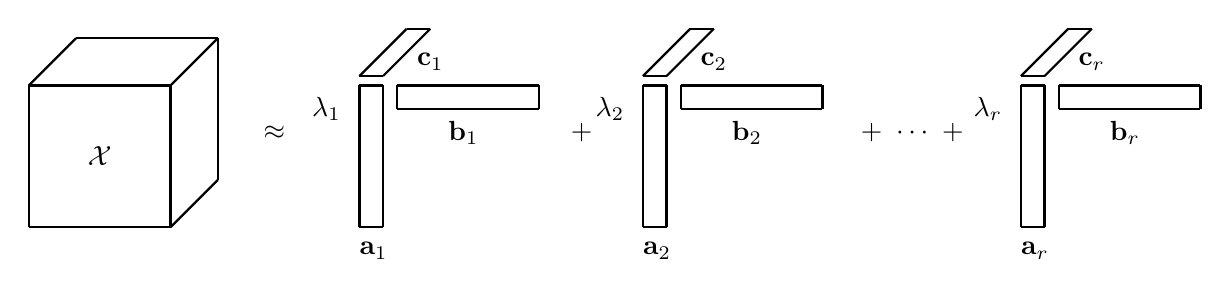
\begin{tikzpicture}[scale=0.6]
%\draw[step=1cm,gray,very thin] (0,0) grid (28,6); %grid lines

\draw node (X) at (1.5, 2.5) {$\T{X}$};
\draw[thick] (0,1) -- (3,1);
\draw[thick] (0,1) -- (0,4);
\draw[thick] (0,4) -- (3,4);
\draw[thick] (3,4) -- (3,1);
\draw[thick] (0,4) -- (1,5);
\draw[thick] (1,5) -- (4,5);
\draw[thick] (3,4) -- (4,5);
\draw[thick] (4,5) -- (4,2);
\draw[thick] (4,2) -- (3,1);

\draw node at (5.2, 3) {$\approx$};

\draw node at (6.3, 3.5) {$\lambda_1$};

\draw node at (7.3, 0.5) {$\V{a}_1$};
\draw[thick] (7,1) -- (7.5,1);
\draw[thick] (7,1) -- (7,4);
\draw[thick] (7,4) -- (7.5,4);
\draw[thick] (7.5,1) -- (7.5,4);

\draw node at (9.2, 3) {$\V{b}_1$};
\draw[thick] (7.8,3.5) -- (7.8,4);
\draw[thick] (7.8,3.5) -- (10.8,3.5);
\draw[thick] (7.8,4) -- (10.8,4);
\draw[thick] (10.8,4) -- (10.8,3.5);

\draw node at (8.5, 4.5) {$\V{c}_1$};
\draw[thick] (7,4.2) -- (7.5,4.2);
\draw[thick] (7,4.2) -- (8,5.2);
\draw[thick] (8,5.2) -- (8.5,5.2);
\draw[thick] (7.5,4.2) -- (8.5,5.2);

\draw node at (11.7, 3) {$+$};

\draw node at (12.3, 3.5) {$\lambda_2$};

\draw node at (13.3, 0.5) {$\V{a}_2$};
\draw[thick] (13,1) -- (13.5,1);
\draw[thick] (13,1) -- (13,4);
\draw[thick] (13,4) -- (13.5,4);
\draw[thick] (13.5,1) -- (13.5,4);

\draw node at (15.2, 3) {$\V{b}_2$};
\draw[thick] (13.8,3.5) -- (13.8,4);
\draw[thick] (13.8,3.5) -- (16.8,3.5);
\draw[thick] (13.8,4) -- (16.8,4);
\draw[thick] (16.8,4) -- (16.8,3.5);

\draw node at (14.5, 4.5) {$\V{c}_2$};
\draw[thick] (13,4.2) -- (13.5,4.2);
\draw[thick] (13,4.2) -- (14,5.2);
\draw[thick] (14,5.2) -- (14.5,5.2);
\draw[thick] (13.5,4.2) -- (14.5,5.2);

\draw node at (18.7, 3) {$+ \ \cdots \ +$};

\draw node at (20.3, 3.5) {$\lambda_r$};

\draw node at (21.3, 0.5) {$\V{a}_r$};
\draw[thick] (21,1) -- (21.5,1);
\draw[thick] (21,1) -- (21,4);
\draw[thick] (21,4) -- (21.5,4);
\draw[thick] (21.5,1) -- (21.5,4);

\draw node at (23.2, 3) {$\V{b}_r$};
\draw[thick] (21.8,3.5) -- (21.8,4);
\draw[thick] (21.8,3.5) -- (24.8,3.5);
\draw[thick] (21.8,4) -- (24.8,4);
\draw[thick] (24.8,4) -- (24.8,3.5);

\draw node at (22.5, 4.5) {$\V{c}_r$};
\draw[thick] (21,4.2) -- (21.5,4.2);
\draw[thick] (21,4.2) -- (22,5.2);
\draw[thick] (22,5.2) -- (22.5,5.2);
\draw[thick] (21.5,4.2) -- (22.5,5.2);
\end{tikzpicture}


\caption{CP decomposition of rank $R$ for a three-dimensional tensor $\T{X}$ \label{fig:3d-cp-decomp}}
\end{figure}
We can represent $\T[]{K}$ in shorthand CP notation as $\T{K} = [\![\V{\lambda};\mat{A}_1,\mat{A}_2, \dots,\mat{A}_d ]\!]$. 
There exists ambiguity in the weighting of the columns of the factor matrices and $\V{\lambda}$ vector.
For simplicity of presentation, we drop the weight vector $\V{\lambda}$ throughout this report and use the representation
$$\T{K} = [\![\mat{A}_1,\mat{A}_2, \dots,\mat{A}_d ]\!].$$

A tensor unfolding is a reshaping of the tensor elements into a matrix; mode-wise unfoldings map tensor fibers of a particular mode to columns of a matrix.
In the case of CP-format tensors like $\T{K}$, the $k$th mode-wise unfolding can be expressed in terms of the factor matrices:
$$\mat{K}_{(k)} = \mat{A}_k (\mat{A}_N \odot \dots \odot \mat{A}_{k+1} \odot \mat{A}_{k-1} \odot \dots \odot \mat{A}_1)^\top,$$
where $\odot$ denotes the Khatri-Rao product.

\subsection{Linear Least Squares Problem}
\label{sec:LS}

In mathematical form, a generic linear least squares problem is given by 
\begin{equation}
\label{eq:LS}
\min_{\mat{X}}||\mat{B} - \mat{X}\mat{A}^\top||_{F}.
\end{equation}
Note that the coefficient matrix $\mat{A}$ appears on the right of the variable matrix, which is the opposite of the standard form.
We use this form to relate to the corresponding least squares problem that arises in the context of computing a CP decomposition.

Several different techniques can be used to solve this problem.
The two we consider here are via the Normal Equations (NE) and by QR decomposition.
The NE specify a (square) linear system of equations and are derived from setting the gradient of the objective function from \cref{eq:LS} to zero, and they involve the Gram of $\mat{A}$ as well as the product $\mat{B}\mat{A}$:
\begin{equation}
\label{eq:NE}
\mat{X}\mat{A}^\top\mat{A} = \mat{B}\mat{A}.
\end{equation}
The NE can be solved via Cholesky factorization of $\mat{A}^\top\mat{A}$ and triangular solves.
The cost of NE depends on the size of $\mat{A}$ and $\mat{B}$. 
For $\mat{A} \in \mathbb{R}^{m \times n}$ and $\mat{B} \in \mathbb{R}^{p \times m}$, the arithmetic complexity of each step of the NE approach is given in \cref{tab:NE-time}.
\begin{table}[!ht]
  \centering
  \begin{tabular}{|c|c|}
    \hline
    Components & Number of flops\\
    \hline
    Compute Gram & $mn^2$ \\
    Compute $\mat{B}\mat{A}$ & $2mnp$\\
    Cholesky factorization & $1/3n^3$ \\
    Back solves & $2pn^2$ \\
    \hline
  \end{tabular}
  \caption{Breakdown of time for using NE to solve \cref{eq:LS} for $\mat{A} \in \mathbb{R}^{m \times n}$ and $\mat{B} \in \mathbb{R}^{p \times m}$}
  \label{tab:NE-time}
\end{table}

In the QR decomposition approach, we first compute the compact QR decomposition $\mat{A} = \mat{Q}\mat{R}$ (so that $\mat{Q}\in \mathbb{R}^{m \times n}$)and then solve the  triangular system
\begin{align}
\label{eq:QR}  
\mat{X} \mat{R}^\top = \mat{B}\mat{Q}.
\end{align}
The time complexity of each step of this approach is given in \cref{tab:QR-time}.
Note that the cost of the QR decomposition assumes that Householder QR is used in the factorization and that the $\mat{Q}$ matrix is formed explicitly.
If $p$ is smaller than $n$, then it is more efficient to leave $\mat{Q}$ in implicit Householder form, reducing the cost of QR to $2mn^2-2/3n^3$.
In this case, we apply $\mat{Q}$ to $\mat{B}$ using Householder transformations, which increases the cost of computing $\mat{B}\mat{Q}$ to $4mnp$. 
%\begin{align}
%  &arg\min_{\mat{X}}||\mat{B} - \mat{X}\mat{A}^\top||_{F}^2 \\
%  &= arg \min_{\mat{X}}||\mat{B} - \mat{X}(\mat{Q}\mat{R})^\top||_{F}^2 \\
%  &= arg \min_{\mat{X}}||\big[\mat{B} - \mat{X}\mat{R}^\top\mat{Q}^\top\big]\big[\mat{Q} \mat{Q}^\bot\big]||_{F}^2 \\
%  &= arg \min_{\mat{X}}||\big[\mat{B}\mat{Q} - \mat{X}\mat{R}^\top \text{    } \mat{B} \mat{Q}^\bot\big]||_{F}^2 \\
%  &= arg \min_{\mat{X}}||\mat{B}\mat{Q} - \mat{X}\mat{R}^\top||_{F}^2 + ||\mat{B}\mat{Q}^\bot||_{F}^2
%\end{align}

\begin{table}[!ht]
  \centering
  \begin{tabular}{|c|c|}
    \hline
    Components & Number of flops\\
    \hline
    Compute QR & $4mn^2 - 4/3n^3$ \\
    Compute $\mat{B}\mat{Q}$ & $2mnp$\\
    N/A & \\
    Back solves & $pn^2$ \\
    \hline
  \end{tabular}
  \caption{Breakdown of time for using QR to solve \cref{eq:LS} for $\mat{A} \in \mathbb{R}^{m \times n}$ and $\mat{B} \in \mathbb{R}^{p \times m}$}
  \label{tab:QR-time}
\end{table}

If $\mat{B}$ has few columns ($p\ll n$), NE is cheaper because of the smaller coefficient in the leading order cost ($mn^2$ vs $2mn^2$). 
However, when $\mat{B}$ has many columns ($p\gg n$), the largest cost is computing $\mat{B}\mat{A}$ for NE and $\mat{B}\mat{Q}$ for QR factorization, which have leading order cost with the same constant ($2mnp$).

Using QR is more numerically stable than NE. 
Let $\kappa = \sigma_1(\mat{A})/\sigma_n(\mat{A})$ be the standard condition number of $\mat{A}$.
If we use QR to solve a least squares problem with a single right hand side; i.e. $\min\|\mat{A}\V{x} - \V{b} \|$, then from \cite[Eq. (19.2)]{trefethen1997numerical} the relative forward error satisfies
\begin{equation}
  \frac{||\V[\tilde]{x} - \V{x}||}{||\V{x}||} = O \biggl(\biggl(\kappa + \frac{\kappa^2\tan\theta}{\eta}\biggr)\epsilon_{mach}\biggr),
\end{equation}
where $\V[\tilde]{x}$ is the computed solution, $\V{x}$ is the exact solution, $\theta$ is the angle between $\mat{A}\V{x}$ and $\V{b}$, and $\eta = \|\mat{A}\|\|\V{x}\|/\|\mat{A}\V{x}\|$.
However, if we use the NE approach, then by \cite[Eq. (19.3)]{trefethen1997numerical} the forward error guarantee can be much larger: 
\begin{equation}
  \frac{||\V[\tilde]{x} - \V{x}||}{||\V{x}||} = O \biggl(\kappa^2 \epsilon_{\text{mach}}\biggr).
\end{equation}
Because of the numerical sensitivity introduced by using the NE approach, the QR approach is much more accurate when $\kappa$ is large (e.g., on the order of $\epsilon_{\text{mach}}^{-1/2}$ or larger).


\subsection{CP-ALS} \label{sec:cp-als}

\subsubsection{CP Optimization Problem}

When computing a rank-$r$ CP approximation $\T{K}$ for a N-way tensor $\T{X}$, we seek to minimize $\| \T{X} - \T{K} \|$, where the tensor norm generalizes the vector 2-norm or the matrix Frobenius norm.
Expressed using \cref{eq:CP}, we have  
$$\min_{\mat{A}_1,\mat{A}_2, \dots,\mat{A}_d} \| \T{X} - \T{K} \|^2 = \min_{\mat{A}_1,\mat{A}_2, \dots,\mat{A}_d} \sum_{i_1=1}^{n_1} \cdots \sum_{i_d=1}^{n_d} \left(\T{X}(i_1,i_2,\dots, i_d) - \sum^{r}_{j=1} \mat{A_1}(i_1,j)\mat{A_2}(i_2,j) \dots \mat{A_d}(i_d,j) \right)^2. $$
However, this is a nonlinear, nonconvex optimization problem and no closed form solution exists. 
We must resort to using iterative methods to approximate a solution \cite{kolda2009tensor}.

\subsubsection{CP-ALS}

One of the most effective algorithms for computing a CP decomposition of a tensor is called Alternating Least Squares (CP-ALS).
The algorithm works as a block coordinate descent method, where each block of variables is a factor matrix.
That is, it alternates over the factor matrices, holding all but one fixed and computing the optimal solution for the variable matrix.

We can solve each subproblem directly because it is a linear least squares problem.
In updating the $n$th factor matrix, we expose the linear least squares problem by unfolding $\T{X}$ and $\T{K}$ along the $k$th mode:
\begin{align}
\label{eq:cp-als-sub}
\min_{\mat{A}_k}||\T{X} - \T{K}|| &= \min_{\mat{A}_k}||\mat{X}_{(k)} - \mat{K}_{(k)}||_F \notag \\ 
&=  \min_{\mat{A}_k}||\mat{X}_{(k)} - \mat{A}_k(\mat{A}_N \odot \dots \odot \mat{A}_{k+1} \odot \mat{A}_{k-1} \odot \dots \odot \mat{A}_1)^\top||_F \notag \\ 
&=  \min_{\mat{A}_k}\|\mat{X}_{(k)}-\mat{A}_k\mat{Z}_k^\top\|_F,
\end{align}
where $\mat{Z}_k=\mat{A}_N \odot \dots \odot \mat{A}_{k+1} \odot \mat{A}_{k-1} \odot \dots \odot \mat{A}_1$.
Note that the coefficient matrix $\mat{Z}_k^\top$ appears on the right of the variable matrix, matching the generic formulation in \cref{eq:LS}.

All of the algorithms we consider in this report are based on CP-ALS, but they differ in how they solve the linear least squares subproblems specified in \cref{eq:cp-als-sub}.

\subsubsection{CP-Rounding}
\label{sec:cp-rounding}

For some applications, we wish to compute a CP decomposition of a matrix that is already in CP format.
That is, we wish to compute a lower-rank representation of the input tensor, sometimes referred to a CP-Rounding.
If $\T{X} \in \mathbb{R}^{n_1 \times \dots \times n_d}$ is a CP-format tensor with rank $s$, it can be written as 
$$\T{X}(i_1,i_2,\dots, i_d) = \sum^{s}_{j=1} \mat{B}_1(i_1,j)\mat{B}_2(i_2,j) \dots \mat{B}_d(i_d,j)$$
with shorthand notation $\T{X} = [\![\mat{B}^{(1)}, \dots ,\mat{B}^{(d)}]\!]$.

In the case the input tensor is in CP format, we can then utilize its special mode-$k$ unfolding representation 
$$\mat{X}_{(k)} = \mat{B}_k(\mat{B}_d \odot \dots \mat{B}_{k+1} \odot \mat{B}_{k-1} \odot \dots \odot \mat{B}_1)^\top$$
when solving the linear least squares problem given in \cref{eq:cp-als-sub}. 
That is, the least squares subproblem is given by 
\begin{equation}
\label{eq:cp-als-sub-ktensor}
\min_{\mat{A}_k}\|\mat{B}_{k}\mat{Y}_k^\top-\mat{A}_k\mat{Z}_k^\top\|_F,
\end{equation}
where $\mat{Y}_k = \mat{B}_N \odot \dots \odot \mat{B}_{k+1} \odot \mat{B}_{k-1} \odot \dots \odot \mat{B}_1$.
This structure can be exploited in different ways depending on how the least squares problem is solved.


\section{Algorithm} \label{sec:algo}

\GB{need to specify notation/dimensions/etc for cost analyses; let's use $n_1 \times \cdots \times n_d$ as tensor dimension, $\bar n$ is the average dimension so that $d\bar n = \sum_k n_k$ and $\hat n$ is the geometric mean so that $\hat n^d = \prod_k n_k$}
The following explanation and tensor notation are assumed having a tensor in$\in \mathbb{R}^{n_1 \times \cdots \times n_d}$.
We define average dimension for that tensor to be $\bar n$ and its geometric mean to be $\hat n$.
$r$ in this section refers to the rank of CP decomposition, and $s$ means the rank for input CP tensor.
\subsection{CP-ALS-NE}


The key to the CP-ALS-NE algorithm is that we will use the normal equations (NE) method to solve the linear least squares problem given by \cref{eq:cp-als-sub} in each mode.
The normal equations for this problem are given by
\begin{equation}
  \label{eq:CP-NE}
  \mat{\hat{A}_k}\mat{Z}_k^\top\mat{Z}_k = \mat{X}_{(k)}\mat{Z}_k.
\end{equation}
The coefficient matrix $\mat{Z}_k^\top\mat{Z}_k$ can be computed as a Hadamard product of Gram matrices of the Khatri-Rao factors:
\begin{equation*}
\mat{Z}_k^\top\mat{Z}_k %= (\mat{A}_N \odot \dots \odot \mat{A}_{k+1} \odot \mat{A}_{k-1} \odot \dots \odot \mat{A}_1)^\top(\mat{A}_N \odot \dots \odot \mat{A}_{k+1} \odot \mat{A}_{k-1} \odot \dots \odot \mat{A}_1) 
= \mat{A}_d^\top \mat{A}_d \hada \cdots \hada \mat{A}_{k+1}^\top\mat{A}_{k+1} \hada \mat{A}_{k-1}^\top\mat{A}_{k-1} \hada \cdots \hada \mat{A}_{1}^\top\mat{A}_{1}.
\end{equation*}
The right hand side matrix $\mat{X}_{(k)}\mat{Z}_k$ can be computed as a matricized tensor times Khatri-Rao product (MTTKRP).
We refer to this standard approach as CP-ALS-NE. Pseudocode for CP-ALS-NE is given in \cref{alg:cp-als-ne}.
\begin{algorithm}[!ht]
  \caption{CP-ALS-NE}
  \label{alg:cp-als-ne}
  %!TEX root = ../Summer-Report.tex

\begin{algorithmic}[1]\footnotesize
    
    \Function{$\{\M{A}_{k}\}=$ CP-ALS-NE}{$\T{X},r$}
      \For{$k = 1, \dots, d$}
        \State Initialize $\mat{A}_k$
        \State $\mat{G}_k = \mat{A}_k^\top\mat{A}_k$ \Comment{compute Gram}
      \EndFor
      \While{not converged}
          \For{$k = 1, \dots, d$}
              \State $\mat{H}_k = \mat{G}_d \hada \cdots \mat{G}_{k+1} \hada \mat{G}_{k-1} \cdots \hada \mat{G}_1$ \Comment{compute $\mat{Z}_k^\top \mat{Z}_k$} \label{l:NE-Hada}
              \State $\mat{M}_k = \mat{X}_{(k)}\mat{Z}_k$ \Comment{MTTKRP} \label{l:NE-mttkrp}
              \State Solve $\mat{A}_k \mat{H}_k = \mat{M}_{k}$ for $\mat{A}_k$ \Comment{via Cholesky} \label{l:NE-solve}
              \State $\mat{G}_k = \mat{A}_k^\top\mat{A}_k$ \Comment{update Gram}   \label{l:NE-Gram}
          \EndFor
      \EndWhile
    \EndFunction
    
  \end{algorithmic}
\end{algorithm}

\subsubsection{Dense Input}

When we have a dense tensor input, the dominant cost of each subiteration comes from the MTTKRP computation of $\mat{M}_k = \mat{X}_{(k)}\mat{Z}_k$ in \cref{l:NE-mttkrp}, which has leading order arithmetic cost of $2\hat n^dr$.
Computing $\mat{H}_k$ in \cref{l:NE-Hada} requires $O(dr^2)$ operations, solving the normal equations in \cref{l:NE-solve} costs $O(r^3+n_kr^2)$, and computing the Gram matrix in \cref{l:NE-Gram} costs $O(n_kr^2)$.
Thus, the sum of an entire CP-ALS-NE iteration (updating all factor matrices once) is given by
\begin{equation*}
2d\hat n^dr + O(d\bar n r^2 + d^2r^2 + dr^3).
\end{equation*}
We note that the leading order term can be reduced to $4\hat n^d r$ and the $O(d^2r^2)$ term can be reduced to $O(dr^2)$ using memoization \cite{phan2013fast}. 
\subsubsection{Kruskal Input}
If the input tensor $\T{X}=[\![\mat{B}^{(1)}, \dots ,\mat{B}^{(d)}]\!]$ is already in Kruskal format (see \cref{sec:cp-rounding}), we can compute the MTTKRP more efficiently using the following identity:
\begin{align*}
  \mat{X}_{(k)}\mat{Z}_k &= \mat{B}_k(\mat{B}_d \odot \dots \odot \mat{B}_{k+1} \odot \mat{B}_{k-1} \odot \dots \odot \mat{B}_1)^\top(\mat{A}_d \odot \cdots \mat{A}_{k+1} \odot \mat{A}_{k-1} \odot \cdots \odot \mat{A}_1) \\
 &= \mat{B}_k(\mat{B}_d^\top\mat{A}_d) \hada \cdots \hada (\mat{B}_{k+1}^\top\mat{A}_{k+1}) \hada (\mat{B}_{k-1}^\top\mat{A}_{k-1}) \hada \cdots \hada (\mat{B}_1^\top\mat{A}_1).  
\end{align*}

With this structure, the algorithm for computing CP decomposition with Kruskal tensor will be  
\begin{algorithm}[!ht]
  \caption{CP-Round-ALS-NE}
  \label{alg:cp-als-ne-k}
  %!TEX root = ../Summer-Report.tex

\begin{algorithmic}[1]
    \Function{$\{\M{A}_{k}\}=$ CP-Round-ALS-NE}{$\{\M{B}_{k}\},r$}
      \For{$k = 1, \dots, d$}
        \State Initialize $\mat{A}_k$
        \State $\mat{G}_k = \mat{A}_k^\top\mat{A}_k$ \Comment{compute Gram}
        \State $\mat{C}_k = \mat{B}_k^\top\mat{A}_k$ \Comment{compute cross product} \label{l:round-ne-cross}
       \EndFor
    
    \While{not converged}
    \For{$k = 1, \dots, d$}
      \State $\mat{H}_k = \mat{G}_d \hada \cdots \mat{G}_{k+1} \hada \mat{G}_{k-1} \cdots \hada \mat{G}_1$ \Comment{compute $\mat{Z}_k^\top \mat{Z}_k$} 
      \State $\mat{D}_k = \mat{B}_k(\mat{C}_d \hada \cdots \mat{C}_{k+1} \hada \mat{C}_{k-1} \cdots\hada \mat{C}_1)$ \Comment{compute $\mat{X}_{(k)}\mat{Z}_n}$ \label{l:round-ne-rhs}
      \State Solve $\mat{A}_k \mat{H}_k = \mat{D}_{k}$ for $\mat{A}_k$ \Comment{via Cholesky} \label{l:NE-K-solve}
      \State $\mat{G}_k = \mat{A}_k^\top\mat{A}_k$ \Comment{update Gram}   \label{l:NE-K-Gram}
      \State $\mat{C}_k = \mat{B}_k^\top\mat{A}_k$ \Comment{update cross product}   \label{l:NE-K-cross}
    \EndFor
    \EndWhile
    \EndFunction
  \end{algorithmic}
  
\end{algorithm}

%The cost when having a Kruskal input is basically the same as dense case. Except for $\mat{X}_{(n)}\mat{Z}_n$ (in \cref{l:round-ne-cross} and \cref{l:round-ne-rhs}) which we only need to do hadamard product requires $O(sn_kr)$ instead of $2\hat{n}^dr$.

When the input is a Kruskal tensor of rank $s>r$, the cost is dominated by the computation of the right hand side of the normal equations.
These costs, incurred in \cref{l:round-ne-rhs,l:NE-K-cross}, are $2n_krs+(d-2)rs$ and $n_krs$ in mode $k$, respectively.
Computing the coefficient matrix of the normal equations occurs in \cref{l:round-ne-gram,l:NE-K-Gram} and has costs $(d-2)r^2$ and $n_kr^2$ in mode $k$.
Solving the normal equations in \cref{l:NE-K-solve} costs $2n_kr^2 + O(r^3)$.
Thus, the sum of an entire CP-Round-ALS-NE iteration (updating all factor matrices once) is given by
\begin{equation*}
4d\bar{n}rs + 3d\bar{n}r^2 + O(d^2rs + d^2r^2 + r^3).
\end{equation*}
We note that the $O(d^2rs+d^2r^2)$ terms can be reduced to $O(drs+dr^2)$ using memoization. 


\subsection{CP-ALS-Explicit-QR}
For CP-ALS-QR approach, it is similar to CP-ALS-NE, but this time more stable QR decomposition is used for solving least square problem instead of NE.
For mode-n least squares problem,
$$\min_{\mat{\hat{A}}_k}||\mat{X}_{(k)} - {\mat{\hat{A}}_k}\mat{Z}^\top_k ||$$
We will first perform QR on each factor matrix in $\mat{Z}_k$, which 
\begin{align}
  \mat{Z}_k &= \mat{A}_d \odot \dots \odot \mat{A}_{k+1} \odot \mat{A}_{k-1} \odot \dots \odot \mat{A}_1 \nonumber \\
  &= (\mat{Q}_d\mat{R}_d) \odot \dots \odot (\mat{Q}_{k+1}\mat{R}_{k+1}) \odot (\mat{Q}_{k-1}\mat{R}_{k-1}) \odot \dots \odot (\mat{Q}_1\mat{R}_1) \nonumber \\
  &= (\mat{Q}_d \otimes \dots \otimes \mat{Q}_{k+1} \otimes \mat{Q}_{k-1} \otimes \dots \otimes \mat{Q}_1)(\mat{R}_d \odot \dots \odot \mat{R}_{k+1} \odot \mat{R}_{k-1} \odot \dots \odot \mat{R}_1)\nonumber  
\end{align}
After that we will perform QR again on $\mat{Q}_0\mat{R}_0= (\mat{R}_d \odot \dots \odot \mat{R}_{k+1} \odot \mat{R}_{k-1} \odot \dots \odot \mat{R}_1)$, so $\mat{Z}_k$ will be
$$\mat{Z}_k = (\mat{Q}_d \otimes \dots \otimes \mat{Q}_{k+1} \otimes \mat{Q}_{k-1} \otimes \dots \otimes \mat{Q}_1)\mat{Q}_0\mat{R}_0$$
The triangular system for QR in this case will be 
\begin{equation}
  \hat{\mat{A}}_k\mat{R}_0^\top = \mat{X}_{(k)}(\mat{Q}_d \otimes \dots \otimes \mat{Q}_{k+1} \otimes \mat{Q}_{k-1} \otimes \dots \otimes \mat{Q}_1)\mat{Q}_0 
  \label{eq:CP-EXP-QR}
\end{equation}
For solving least square problem, we will first apply kronecker product of Qs $\mat{Q}_d \otimes \dots \otimes \mat{Q}_{k+1} \otimes \mat{Q}_{k-1} \otimes \dots \otimes \mat{Q}_1$ into $\mat{X}_{(k)}$
$$\mat{Y}_{(k)} = \mat{X}_{(k)}(\mat{Q}_d \otimes \dots \otimes \mat{Q}_{k+1} \otimes \mat{Q}_{k-1} \otimes \dots \otimes \mat{Q}_1)$$
Then use backslash to solve the linear system
\begin{equation}
  \hat{\mat{A}}_k = \mat{R}_0^\top \text{\textbackslash} \mat{Y}_{(k)}\mat{Q}_0
\end{equation}
Sample pseudocode for CP-ALS-QR is showed in \cref{alg:cp-als-qr}
\begin{algorithm}
  \caption{CP-ALS-QR-Exp}
  \label{alg:cp-als-qr}
  \begin{algorithmic}[1]
    \Function{$[\bm{\lambda},\M{A}_{n}]=$ CP-ALS}{$\T{X},R$}
      \State Setup factor matrices  $\mat{A}_1$, $\mat{A}_2$, $\dots$, $\mat{A}_n$
      \State Compute QR decomposition for factor matrices $\mat{Q}_N\mat{R}_N, \dots \mat{Q}_1\mat{R}_1$
      \While{not converge}
      \For{$n = 1, \dots, N$}
      %\State Compute QR factorization $\mat{Q}_0\mat{R}_0$ for Khatri-Rao product of $\mat{R}_N, \dots, \mat{R}_1$
      \State $[\mat{Q}_0,\mat{R}_0] = \Call{QR}{\mat{R}_N \odot \cdots \odot \mat{R}_1}$
      \State $\T{Y} =  \T{X} \times_1 \mat{Q}_1^\top \dots \times_{n-1} \mat{Q}_{n-1}^\top \times_{n+1} \mat{Q}_{n+1}^\top \dots \times_N \mat{Q}_N^\top$ \Comment{Multi-TTM} \label{l:TTM}
      \State $\mat{U}_n = \mat{Y}_{(n)}\mat{Q}_0$ \label{l:apply}
      \State Solve $\mat{\hat{A}_n} = \mat{R}_0^\top \text{\textbackslash} \mat{U}_n$
      \State Update $\mat{A}_n$ and $\bm{\lambda}$
      \State Update QR for $\mat{A}_n = \mat{Q}_n\mat{R}_n$      
      \EndFor
      \EndWhile
    \EndFunction
  \end{algorithmic}
\end{algorithm}

\subsubsection{Dense Input}
%The difference between dense and Kruskal tensor is the computation of $\mat{Y}_{(k)}$. 
For dense input, the computation of each subiteration is dominated by \cref{l:EXP-TTM}, which is a multiple tensor-times-matrix (Multi-TTM) computation to form $\T{Y}$ with cost
$2\hat{n}^dr+O(\hat{n}^{d-1}r^2 + \cdots + \hat{n}r^d)$, where we assume the Multi-TTM is performed in order of largest mode to smallest (the largest mode is at least the geometric mean).
The cost of the QR of the Khatri-Rao product of triangular factors in \cref{l:EXP-QR-R} is $4r^{d+1}+O(r^3)$, where we assume $\mat{Q}_0$ is formed explicitly.
The cost of multiplying $\mat{Q}_0$ by $\mat{Y}_{(k)}$ in \cref{l:apply} is $2n_kr^d$.
Solving the triangular system in \cref{l:cp-als-q-exp:solve} costs $n_kr^2$, and computing the QR of the factor matrix in \cref{l:cp-als-q-exp:updateQR} is $4n_kr^2+O(r^3)$, where again we form the orthogonal factor explicitly.
%
%$$\T[]{Y} = \T[]{X} \times_1 \mat{Q}_1^\top \times \dots \times_{k-1} \mat{Q}_{k-1}^\top \times_{k+1}\mat{Q}_{k+1}^\top \times \dots \times_d \mat{Q}_d^\top$$
%and use matricized tensor $\mat{Y}_{(k)}$ times $\mat{Q}_0$.
%The computation of QR for factor matrices in \cref{l:qr_factor_q} takes $(d-2)r^2\bar{n}$. 
%The QR for Khatri-Rao product of $\mat{R}$ in \cref{l:EXP-QR-R} takes $O(r^{d+1})$ overall. 
%The cost for doing Multi-TTM will be $\hat{n}^dr$ and $\mat{U}_k = \mat{Y}_{(k)}\mat{Q}_0$ in \cref{l:apply} will be $\bar{n}r^d$.
Overall, the cost of updating factor matrices along all modes for CP-ALS-QR-Exp is
$$2d\hat{n}^dr + O(d\hat{n}^{d-1}r^2 + \cdots + d\hat{n}r^d + d\bar{n}r^d+ dr^{d+1} + d\bar{n}r^2 + dr^3 ).$$
Note that the leading order term (and several others) can be reduced by a factor of $O(d)$ using memoization \cite{KR19}.

\subsubsection{Kruskal Input}
If we have a Kruskal tensor input, the computation of right hand side will be more efficient by applying cross product for $\mat{Q}_k^\top\mat{B}_k$
\begin{equation}
  \mat{Y}_{(k)}\mat{Q}_0= \mat{B}_k(\mat{Q}_d^\top\mat{B}_d \odot \cdots \odot \mat{Q}_{k+1}^\top\mat{B}_{k+1} \odot \mat{Q}_{k-1}^\top\mat{B}_{k-1} \odot \cdots \odot \mat{Q}_1^\top\mat{B}_1)^\top\mat{Q}_0 \nonumber
\end{equation}
We can treat $\mat{Q}_0$ as a matricized tensor and we can compute this as MTTKRP and a small matrix multiplication.

\begin{algorithm}[!ht]
  \caption{CP-Round-ALS-QR-Exp}
  \label{alg:cp-als-qr-k}
  \begin{algorithmic}[1]
    \Function{$\{\M{A}_{n}\}=$ CP-ALS-EXPLICIT-QR-KRUSKAL}{$\T{X},r$}
      \For{$l = 1,\dots, d$}
      \State Init $\mat{A}_l$
      \State $[\mat{Q}_l,\mat{R}_l] = \Call{QR}{\mat{A}_l}$ \Comment{Factor QR}
        \State $\mat{C}_l = \mat{B}_l^\top\mat{Q}_l$ \Comment{Update $\mat{Y}_{(k)}$} \label{l:EXP-K-Apply}

      \EndFor
      \While{not converge}
      \For{$k = 1, \dots, d$}
      
      \State $\mat{U}_k = (\mat{C}_d \odot \cdots \mat{C}_{k+1} \odot \mat{C}_{n-1} \odot \cdots \mat{C}_1)\mat{Q}_0$ \Comment{MTTKRP}
      \State $\mat{U}_k = \mat{B}_k\mat{U}_k$ \Comment{matrix Mult}
      \State Solve $\mat{\hat{A}_k}\mat{R}_0^\top = \mat{U}_k$ for $\mat{A}_k$ \Comment{via TRSM}
      \State $[\mat{Q}_k,\mat{R}_k] = \Call{QR}{\mat{A}_k}$ \Comment{Update $\mat{Q}_k\mat{R}_k$}     
      \EndFor
      \EndWhile
    \EndFunction
  \end{algorithmic}
\end{algorithm}

%The cost for this algorithm is also similar to the code in dense case. However, in \cref{l:EXP-K-Apply}, the cost is $O(snr)$.
%and in \cref{l:EXP-mttkrp} the MTTKRP dominates the cost which is $(\hat{n}^dr)$.
In the case of Kruskal input, the costs of \cref{l:cp-round-als-exp-qr,l:cp-round-qr-solve,l:cp-round-qr-updateqr} are identical to the corresponding lines in \cref{alg:cp-als-qr}, with combined cost of $4r^{d+1}+9n_kr^2+O(r^3)$ in mode $k$.
The cost of \cref{l:EXP-mttkrp}, which we implement as an MTTKRP, is $2r^ds$.
The cost of the matrix multiplications in \cref{l:exp-finish-rhs,l:EXP-K-update-cross} together is $4n_krs$.
Thus, the overall cost of CP-Round-ALS-QR-Exp is
$$ 2dr^ds + 4dr^{d+1} + O(d\bar{n}rs+d\bar{n}r^2 + r^3).$$
Again, it is possible to reduce the leading order costs by a factor of $O(d)$ via memoization.

\subsection{CP-ALS-Pairwise-QR}
\subsubsection{Algo}
There is also a new QR-based method instead of computing QR on $(\mat{R}_d \odot \dots \odot \mat{R}_1)$, it compute QR for Khatri-Rao product of two matrices $\mat{R_n} \odot \mat{R}_{n-1}$.
It avoids the formation of $\mat{Q}_0\mat{R}_0$ which its cost is exponential respect to the size of input tensor.
Doing QR on factor matrices is the same.
$$\mat{Z}_k = (\mat{Q}_d \otimes \dots \otimes \mat{Q}_{k+1} \otimes \mat{Q}_{k-1} \otimes \dots \otimes \mat{Q}_1)(\mat{R}_d \odot \dots \odot \mat{R}_{k+1} \odot \mat{R}_{k-1} \odot \dots \odot \mat{R}_1)$$
But this time we will first do QR for $\mat{R}_d \odot \mat{R}_{d-1} = \mat{Q}_{A}\mat{R}_A$ and Khatri-Rao product of $\mat{R}$ will be 
$$\mat{Q}_{A_{d-1}}\mat{R}_{A_{d-1}} \odot \mat{R}_{d-2} \odot \dots \odot \mat{R}_{k+1} \odot \mat{R}_{k-1} \odot \dots \odot \mat{R}_1$$
We will use the same technique in representing $\mat{Z}_k$, which this will transform into 
$$(\mat{Q}_{A_{d-1}} \otimes \dots \otimes \mat{I}_d \otimes \mat{I}_d \otimes \dots  \otimes  \mat{I}_d)(\mat{R}_{A_{d-1}} \odot \dots \odot \mat{R}_{k+1} \odot \mat{R}_{k-1} \odot \dots \odot \mat{R}_1)$$
By continuing doing this pariwise QR decomposition on $\mat{R}$, we eventually will have a bunch of new QR representations like
$$\mat{V}_d = \underbrace{(\mat{Q}_{A_{d-1}} \otimes \dots  \otimes  \mat{I}_d)}_{d-2}\underbrace{(\mat{Q}_{A_{d-2}} \otimes \dots \otimes \mat{I}_d)}_{d-3} \cdots (\mat{Q}_{A_{2}} \otimes \mat{I}_d) \mat{Q}_{A_{1}}\mat{R}_{A_{1}}$$
where $\mat{Z}_k$ will be 
$$\mat{Z}_k = (\mat{Q}_d \otimes \dots \otimes \mat{Q}_{k+1} \otimes \mat{Q}_{k-1} \otimes \dots \otimes \mat{Q}_1) (\mat{Q}_{A_{d-1}} \otimes \dots  \otimes  \mat{I}_d)(\mat{Q}_{A_{d-2}} \otimes \dots \otimes \mat{I}_d) \cdots (\mat{Q}_{A_{2}} \otimes \mat{I}_d) \mat{Q}_{A_{1}}\mat{R}_{A_{1}}$$
We can 
The sample pseudocode is showed in \cref{alg:cp-als-pairwise-qr} 
\begin{algorithm}
  \caption{CP-ALS-QR-Imp}
  \label{alg:cp-als-pairwise-qr}
  \begin{algorithmic}[1]
    \Function{$[\bm{\lambda},\M{A}_{n}]=$ CP-ALS}{$\T{X},R$}
      \State Setup factor matirces  $\mat{A}_1$, $\mat{A}_2$, $\dots$, $\mat{A}_n$
      \State Compute QR decomposition for factor matrices $\mat{Q}_N\mat{R}_N, \dots \mat{Q}_1\mat{R}_1$
      \While{not converge}
      \For{$n = 1, \dots, N$}
      \State Compute pairwise QR factorization $(\mat{Q}_{A_{N-1}} \otimes \dots  \otimes  \mat{I}_N) \dots \mat{Q}_{A_{1}}\mat{R}_{A_{1}}$ for each $\mat{R}_N, \dots, \mat{R}_1$
      \State TTM with Kruskal format $\mat{Y}_{(n)} = \mat{B}_1\mat{Q}^\top_1 \odot \dots \odot \mat{B}_{n-1}\mat{Q}^\top_{n-1}\odot \mat{B}_{n+1}\mat{Q}^\top_{n+1} \odot \dots \odot \mat{B}_N\mat{Q}^\top_N$
      \State Apply pairwise QR on $\mat{Y}_n\mat{Q}_{A_{N-1}}^\top  = (\mat{Q}_{A_{N-1}}^\top(\mat{Q}_N\mat{B}_N \odot \mat{Q}_{N-1}\mat{B}_{N-1}) \odot \dots \odot  \odot \mat{Q}_{1}\mat{B}_{1})^\top\mat{B}_n $
      
      \State Solve $  \mat{\hat{A}}_n = \mat{R}^\top_{A_1} \text{\textbackslash} \mat{B}^\top_M\mat{Q}_M\mat{B}_n $
      \State Update $\mat{A}_n$ and $\bm{\lambda}$
      \State Update QR for $\mat{A}_n = \mat{Q}_n\mat{R}_n$      
      \EndFor
      \EndWhile
    \EndFunction
  \end{algorithmic}
\end{algorithm}


\subsubsection{Dense Input}

The cost of the factor matrix QR in \cref{l:cp-als-q-exp:updateQR} is $4n_kr^2+O(r^3)$ in mode $k$.
The cost of the Multi-TTM in \cref{l:pairwise-TTM} is the same as in \cref{alg:cp-als-qr}: $2\hat{n}^dr+O(\hat{n}^{d-1}r^2 + \cdots + \hat{n}r^d)$.
The permutation has no arithmetic cost, though in practice it may take significant time due to the high relative cost of memory movement.
The pairwise QR decompositions together cost $4(d-2)r^4 + O(dr^3)$ for mode $k$, and applying the pairwise orthogonal factors via TTM costs a total of $2n_kr^d+2n_kr^{d-1}+\cdots+2n_kr^3$.
The triangular solve in \cref{l:cp-als-q-exp:solve} costs $n_kr^2$.
Thus, the total cost of a full iteration (updating each factor matrix once) of CP-ALS-QR-Imp is
$$ 2d\hat{n}^d + 2d\bar{n}r^d + 4d^2r^4 + O(d\hat{n}^{d-1}r^2 + d\bar{n}r^{d-1}). $$
The leading order cost can be reduced by a factor of $O(d)$ via memoization \cite{KR19}.

\subsubsection{Kruskal Input} \label{sec:QR-PW-k}

With Kruskal input, we can use the Kruskal structure $\mat{X}_{(k)} = \mat{B}_{k}(\mat{B}_{d} \odot \dots \odot \mat{B}_{k+1} \odot \mat{B}_{k-1}  \odot \dots \odot \mat{B}_{1})^\top$. 
Applying $\mat{Q}$ into $\mat{X}_k$. 
This gives us
\begin{align}
  \mat{Y}_k &= (\mat{B}_{k}(\mat{B}_{d} \odot \dots \odot \mat{B}_{k+1} \odot \mat{B}_{k-1}  \odot \dots \odot \mat{B}_{1})^\top)(\mat{Q}_d \otimes \dots \otimes \mat{Q}_{k+1} \otimes \mat{Q}_{k-1} \otimes \dots \otimes \mat{Q}_1) \nonumber \\
  &= \mat{B}_k(\mat{Q}_d^\top\mat{B}_d \odot \cdots \odot \mat{Q}_{k+1}^\top\mat{B}_{k+1} \odot \mat{Q}_{k-1}^\top\mat{B}_{k-1} \odot \cdots \odot \mat{Q}_1^\top\mat{B}_1)^\top \nonumber
\end{align}
On following step, we will apply that set of kronecker $\mat{Q}$ into $\mat{Y}_k$ in similar pairwise way.
\begin{align}
  \mat{Y}_k &= \mat{B}_k(\mat{Q}_d^\top\mat{B}_d \odot \cdots \odot \mat{Q}_{k+1}^\top\mat{B}_{k+1} \odot \mat{Q}_{k-1}^\top\mat{B}_{k-1} \odot \cdots \odot \mat{Q}_1^\top\mat{B}_1)^\top \nonumber \\
      &= \mat{B}_k((\mat{Q}_d^\top\mat{B}_d \odot \mat{Q}_{d-1}^\top\mat{B}_{d-1}) \odot \dots \odot \mat{Q}_{k+1}^\top\mat{B}_{k+1}\odot \mat{Q}_{k-1}^\top\mat{B}_{k-1} \odot \dots \odot \mat{Q}_{1}^\top\mat{B}_{1})^\top \nonumber      \\
      \mat{Y}_k\mat{Q}_{A_{d-1}}  &= \mat{B}_k(\mat{Q}_{A_{d-1}}((\mat{Q}_d^\top\mat{B}_d \odot \mat{Q}_{d-1}^\top\mat{B}_{d-1}) \odot \dots \odot \mat{Q}_{k+1}^\top\mat{B}_{k+1}\odot \mat{Q}_{k-1}^\top\mat{B}_{k-1} \odot \dots \odot \mat{Q}_{1}^\top\mat{B}_{1}))^\top \nonumber      \\
      & \vdots \nonumber \\
    \mat{U}_k  &= \mat{B}_k(\mat{Q}_M^\top\mat{B}_M)^\top \nonumber  
\end{align}
Notice that we only have to do one matrix multiplication once a time because when use the same property, one matrix times an identity matrix will still be itself.
We can solve this linear system
\begin{equation}
  \mat{\hat{A}}_k\mat{R}_{A_1}^\top = \mat{U}_k 
\end{equation}
The algorithm for CP-ALS-Pairwise-QR in Kruskal input will be
\begin{algorithm}
  \caption{CP-Round-ALS-QR-Imp}
  \label{alg:cp-als-pairwise-qr-kruskal}
  %!TEX root = ../Summer-Report.tex

\begin{algorithmic}[1]
    \Function{$\{\M{A}_{k}\}=$ CP-Round-ALS-QR-Imp}{$\{\M{B}_{k}\},r$}
      \For{$k = 1, \dots, d$}
        \State Initialize $\mat{A}_k$
        \State $[\mat{Q}_k,\mat{R}_k] = \Call{QR}{\mat{A}_k}$ \Comment{compute QR} 
        \State $\mat{C}_k = \mat{Q}_k^\top\mat{B}_k$ \label{l:Pair-K-Apply} \Comment{compute cross product}  
      \EndFor
      \While{not converge}
        \For{$k = 1, \dots, d$}
          \IfThenElse{$k \neq 1$}{$a=1$}{$a=2$} \Comment{set starting index}
          \State $\mat{R}_0 = \mat{R}_a$, $\mat{D}_k = \mat{C}_a$ \Comment{initialize pairwise results}
          \For{$\ell = 1, \dots, d$} 
            \If{$\ell\neq k \textbf{ and }\ell\neq a$}
              \State $[\mat{Q}_0,\mat{R}_0] = \Call{QR}{\mat{R}_\ell \odot \mat{R}_0}$ \label{l:pair-QR-R} \Comment{pairwise QR}
              \State $\mat{D}_k = (\mat{C}_\ell \odot \mat{D}_k)^\top\mat{Q}_0$ \Comment{pairwise apply}
            \EndIf
          \EndFor
          \State $\mat{U}_k = \mat{B}_k\mat{D}_k$ \Comment{via matrix multiplication}
          \State Solve $  \mat{A}_k\mat{R}_0^\top = \mat{U}_k$ for $\mat{A}_k$ \Comment{via triangular solve}    
          \State $[\mat{Q}_k,\mat{R}_k] = \Call{QR}{\mat{A}_k}$ \Comment{update QR}   
          \State $\mat{C}_k = \mat{Q}_k^\top\mat{B}_k$ \label{l:Pair-K-update} \Comment{update cross product}  
        \EndFor
      \EndWhile
    \EndFunction
  \end{algorithmic}
\end{algorithm}


For Kruskal input of rank $s$, we first consider the costs of the factor matrix QR decompositions and applying the individual orthogonal factors.
In mode $k$, the cost of the QR in \cref{l:Pair-K-update} is $4n_kr^2$, and the cost of applying the explicit orthogonal factor to the corresponding input factor matrix is $2n_krs$.
Performing the pairwise QR decompositions and applying the explicit orthogonal factors occurs in \cref{l:pair-QR-R,l:pair-QR-Rapply}.
For each subiteration, the cost of the two operations, which are both performed $d-2$ times, is $4dr^4+2dr^3s+O(r^4)$.
The final multiplication and triangular solve in \cref{l:Pair-K-matmul,l:Pair-K-solve} together cost $2n_krs+n_kr^2$.
Performing a full iteration and updating each factor matrix once has total cost
$$ 4d\bar{n}rs + 5d\bar{n}r^2 + 2d^2r^3s + 4d^2r^4 + O(r^4). $$
The terms involving factors of $d^2$ can likely be reduced by a factor of $d$ via memoization.

\subsection{Complexity}
Given a dense tensor has the properties at the beginning of this section. 
If we want to do the rank-$r$ CP Decomposition for different ALS methods, the distribution of time is presented in \cref{tab:dense_its_part}


\begin{table}[!ht] 
  \centering
  \begin{tabular}{|c|c|c|c|c|c|}
    \hline
    \multicolumn{2}{|c|}{\textbf{Normal Equations}} & \multicolumn{2}{|c|}{\textbf{Explicit QR}} & \multicolumn{2}{|c|}{\textbf{Implicit QR}} \\
    \hline
    Component & Cost & Component & Cost & Component & Cost \\
    \hline
    Compute RHS &$2d \hat{n}^d r$ &Multi-TTM &$2d\hat n^d r$  & Multi-TTM &$2d\hat n^d r$  \\
    Compute Gram & $d^2r^2 + 3d \bar{n} r^2$&QR on factor matrices & $4d \bar n r^2$ & QR on factor matrices & $4d \bar n r^2$\\
    N/A& &Compute $\mat{Q}_0$ & $4dr^{d+1}$& Compute $\tilde{\mat{Q}}\tilde{\mat{R}}$& $4d^2r^4$\\
    N/A & &Apply $\mat{Q}_0$& $2d\bar n r^d$& Apply $\tilde{\mat{Q}}\tilde{\mat{R}}$& $2d\bar n r^d$\\
    \hline
  \end{tabular}
  \caption{Breakdown of main component when using NE, explicit QR, implicit QR along all modes}
  \label{tab:dense_its_part}
\end{table}






If we already have a Kruskal tensor as input, the distribution of time on different method is showed in \cref{tab:kruskal_its_part}.
\begin{table}[!ht] 
  \centering
  \begin{tabular}{|c|c|c|c|c|c|}
    \hline
    \multicolumn{2}{|c|}{\textbf{Normal Equations}} & \multicolumn{2}{|c|}{\textbf{Explicit QR}} & \multicolumn{2}{|c|}{\textbf{Implicit QR}} \\
    \hline
    Component & Cost & Component & Cost & Component & Cost \\
    \hline
    Compute RHS &$4d\bar n rs$ &  Cross Product&$2d\bar n rs$  & Cross Product &$2d\bar n rs$  \\
    Compute Gram & $d^2r^2+3d\bar n r^2$&QR on factor matrices & $4d \bar n r^2$ & QR on factor matrices & $4d \bar n r^2$\\
    N/A& &Compute $\mat{Q}_0$ & $4dr^{d+1}$& Compute $\tilde{\mat{Q}}\tilde{\mat{R}}$& $4d^2r^4$\\
    N/A & &Apply $\mat{Q}_0$& $2d\bar nrs$& Apply $\tilde{\mat{Q}}\tilde{\mat{R}}$& $2d \bar n rs$\\
    \hline
  \end{tabular}
  \caption{Breakdown of main component given Kruskal tensor input using NE, explicit QR, and implicit QR along all modes}
  \label{tab:kruskal_its_part}
\end{table}


  




\section{Experimental Results} \label{sec:result}


\subsection{Sine of Sums Tensor}

To test the accuracy and efficiency of the QR-based method, we use a discretization of sine of sums: $\sin(x_1+\dots+ x_d)$.
Repeated use of the textbook sine of sums identity for two variables, we obtain a $2^{d-1}$-term separated representation of the function.
For example, 
\begin{equation*}
\begin{split}
\sin(x_1+x_2+x_3) = \sin(x_1)\cos(x_2)\cos(x_3)+\cos(x_1)\cos(x_2)\sin(x_3) \\
+\cos(x_1)\sin(x_2)\cos(x_3) - \sin(x_1)\sin(x_2)\sin(x_3).
\end{split}
\end{equation*}
\GB{Shouldn't there be two negative terms in this expression?}
As described in previous work \cite{BM02,MVLB23}, there exists a $d$-term separated representation of the form
$$\sin\left(\sum^d_{j=1}x_j\right) = \sum^d_{j=1}\sin(x_j)\prod^d_{k=1,k\neq j}\frac{\sin(x_k - \alpha_k -\alpha_j)}{\sin(\alpha_k - \alpha_j)}$$
for all choices of  ${\alpha_j}$ such that $\sin(\alpha_k - \alpha_j) \neq 0$ for all $j \neq k$.
Our goal is to compute this much more efficient $d$-term representation using the $2^{d-1}$-term representation numerically using discretized representations of the functions.

\subsection{Single Least Squares Problem}

%We can somehow treat this sine of sum be a N-mode tensor $\T{X} \in \mathbb{R}^{n \times \dots \times n}$, and each term of exponential representation corresponds to a rank $2^{d-1}$ CP decomposition. 
%It is also possible to have a rank $n$ CP decomposition by the linear representation mentioned above. 
%This representation can be ill-conditioned if $\alpha_k \rightarrow \alpha_j$.
%In the actual problem setup, we make $a_k$ and $a_j$ to be evenly spaced between $\frac{\pi}{d}\frac{(d-1)}{100}$. 

The goal for this test is to see how the speed and accuracy of different algorithms will change when varying condition number $K$.
We first created bunch of ktensors given different $d$. The least squares problems here are trying to approximate the last factor matrix in exponential representation. Comparing the relative error between approximated matrix and the factor matrix we formed in linear representation through built function. 

Based on the problem setup, we measured the forward error by varying the distance between $\alpha_j$ and $\alpha_{j+1}$.
We believed that this will change condition number which also lead to changes in accuracy in \cref{tab:LS_err}. 

\begin{table}[ht!] 
  \centering
  \begin{tabular}{|c|c|c|c|c|c|c|}
    \hline
    $d$ & $n$ & $|\alpha_j-\alpha_{j+1}|$ & $\kappa$ & NE Fwd Err & QR Exp Fwd Err & QR PW Fwd Err \\
    \hline
    3 & 50 & \texttt{1e0}  & \texttt{1.51e0}  & \texttt{3.64e-16} & \texttt{1.44e-15} & \texttt{5.07e-16} \\
    3 & 50 & \texttt{1e-1} & \texttt{5.02e2}  & \texttt{6.12e-14} & \texttt{3.70e-15} & \texttt{5.74e-16} \\
    5 & 50 & \texttt{1e-1} & \texttt{7.38e3}  & \texttt{9.80e-11} & \texttt{9.70e-15} & \texttt{1.85e-15}\\
    3 & 50 & \texttt{1e-2} & \texttt{4.77e5}  & \texttt{1.32e-08} & \texttt{5.40e-13} & \texttt{8.99e-15} \\
    5 & 50 & \texttt{1e-2} & \texttt{3.71e8}  & \texttt{3.51e-01} & \texttt{4.87e-12} & \texttt{1.27e-14}\\
    3 & 50 & \texttt{1e-4} & \texttt{4.77e11} & \texttt{8.89e-01} & \texttt{8.43e-09} & \texttt{1.31e-12} \\
    5 & 50 & \texttt{1e-3} & \texttt{3.64e13} & \texttt{1.00e00}  & \texttt{9.74e-07} & \texttt{1.94e-09}\\
    \hline
  \end{tabular}
  \caption{Forward Error when varying $|\alpha_j-\alpha_{j+1}|$ for NE, QR Imp, and QR Exp}
  \label{tab:LS_err}
\end{table}
We can observe that as the distance decreases, the condition number increases, and the forward error for NE changes a lot.

Figure indicating speed differences is showed in \cref{fig:LS_problem_line}.
\begin{figure}[ht!]
  \begin{center}
    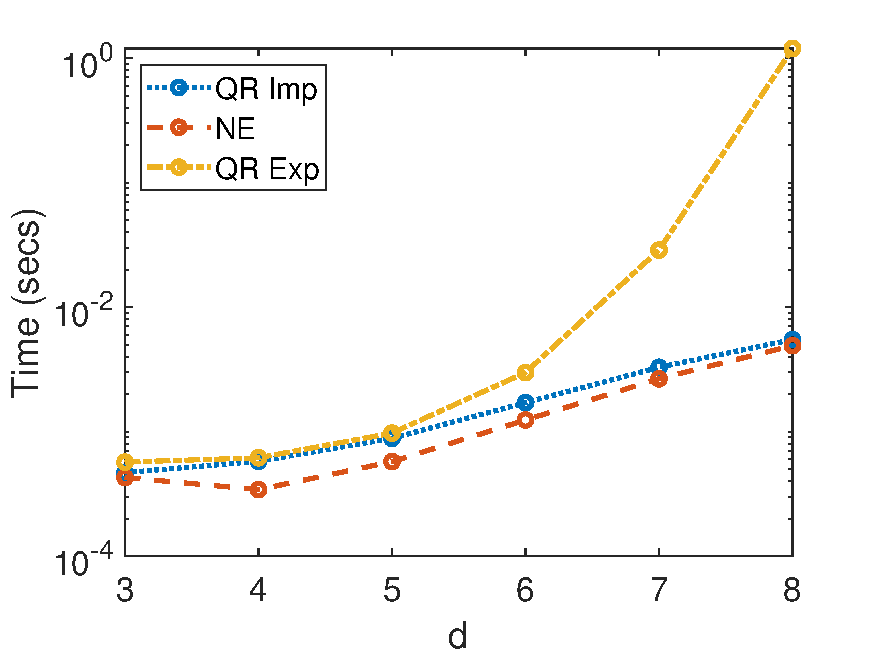
\includegraphics[scale = 0.7]{lineplot_p.pdf}
    \caption[Figure]{runtime for NE, QR Imp and QR Exp in different modes \label{fig:LS_problem_line}}
  \end{center}
\end{figure}


For speed figure \cref{fig:LS_problem_line}, the time for doing QR Exp increases exponential respect to number of modes.
Wheras the time for NE and QR Imp increase much slower and sometimes QR Imp is actually faster than NE.
This is because the time for computing QR on $\mat{R}_N \odot \dots \odot \mat{R}_1$ is exponential to $d$.
In some sense, QR Exp will not be a good choice to solve least square problem if the number of modes is to high.

In the next breakdown figure \cref{fig:LS_problem_breakdown}, we will later see where the majority time goes.
\begin{figure}[ht!]
  \begin{center}
    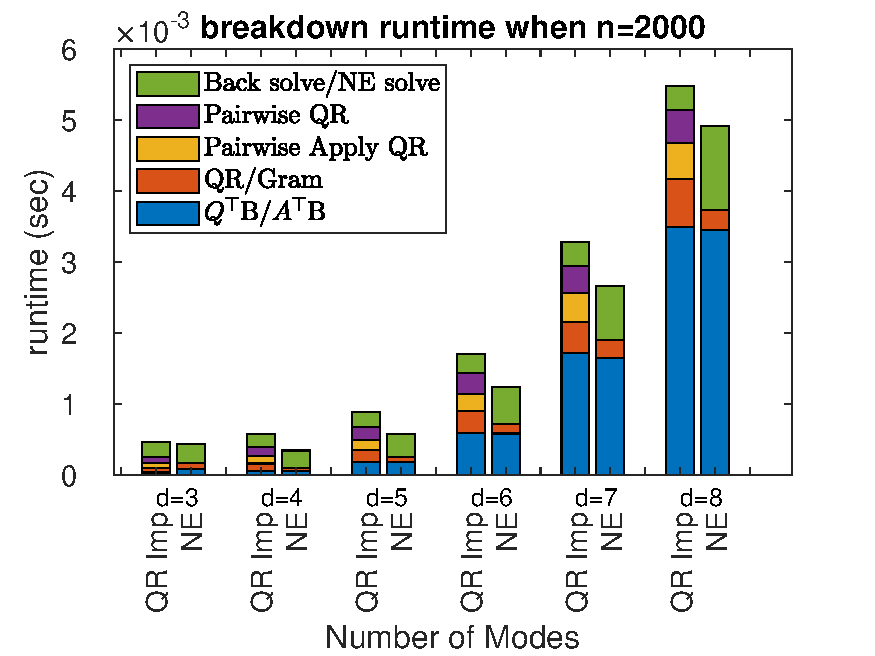
\includegraphics[scale = 0.8]{breakdown_p.pdf}
    \caption[Figure]{Breakdown of runtime for NE and QR Imp\label{fig:LS_problem_breakdown}}
  \end{center}
\end{figure}

In \cref{fig:LS_problem_breakdown} we can see that the time to apply gram matrices and factor Q matrices to RHS is about the same for each approach.
In QR Imp, the computation for factor QR takes a little bit more time than computing the gram matrices and it has two extra steps for doing QR on Khatri-Rao R.
So we don't really expect it will be faster than NE approach. 
However, one thing to notice that the time for solving linear system on NE approach takes much longer than QR Imp approach.
This is because MATLAB will perform SVD solve if the system condition number is too high.
It will be slower then Cholesky solve performed in QR Imp.

\subsection{CP-ALS}

In the next step, we put QR Imp into CP-ALS which further compare the runtime and accuracy to CP-Round-ALS-NE and CP-Round-ALS-QR-Exp. 
This is known that cost of QR Exp is exponential to $d$, which will take longer than the rest when solving a LS problem.
This case is further amplified when doing CP-ALS with more computation needed.
\begin{figure}[ht!]
  \begin{center}
    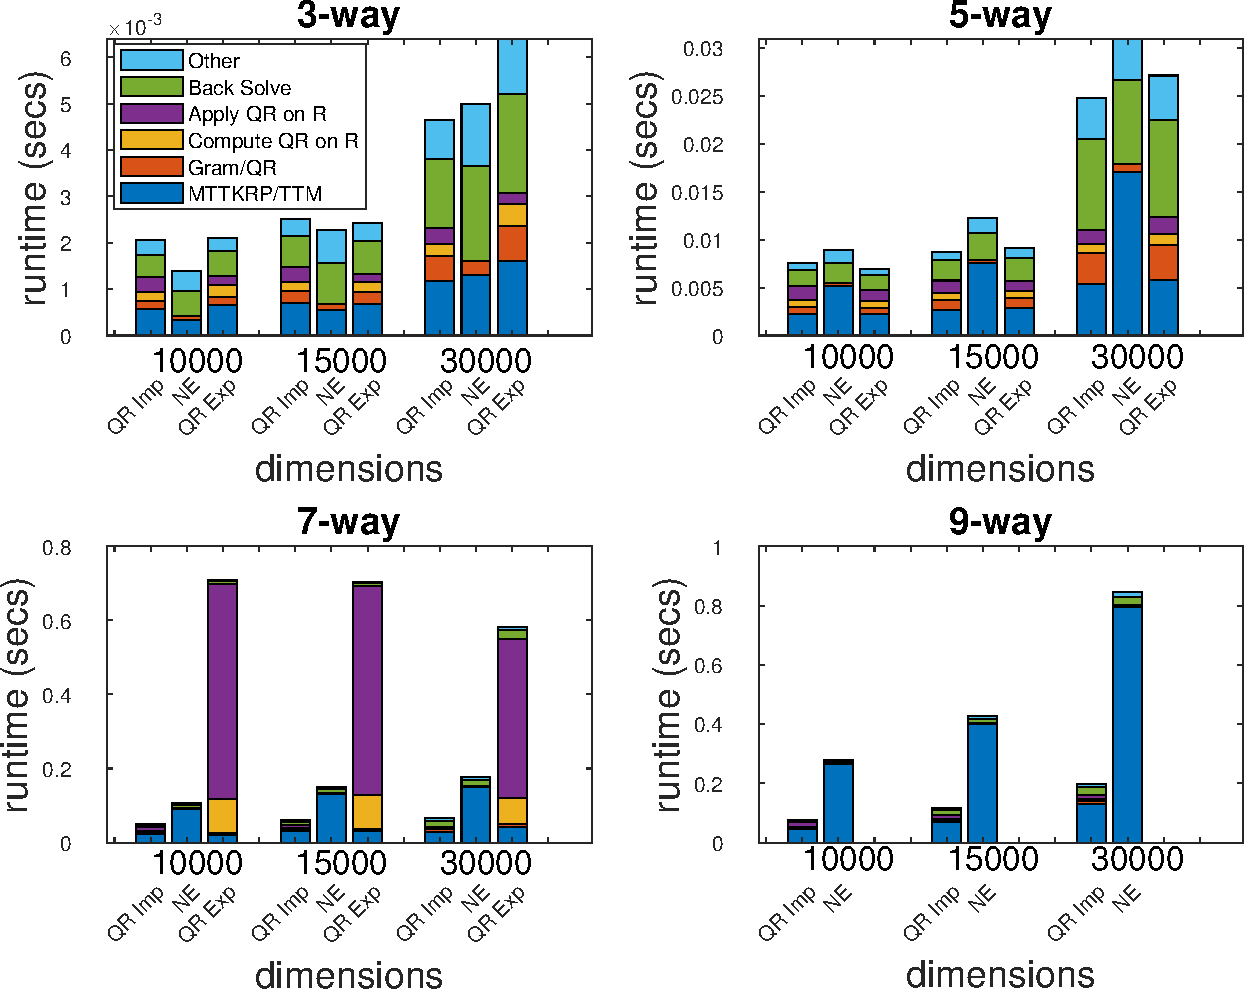
\includegraphics[scale = 0.7]{Fig_kt.pdf}
    \caption[Figure]{runtime for NE, QR Imp and QR Exp in different dimensions in each subinteration \label{fig:runtime}}
  \end{center}
\end{figure}


As showed in \cref{fig:runtime}, we created 3-way, 5-way, 7-way and 9-way ktensors to show time distributions for each component.
We also varied its dimensions $n$ to see how each approach cost changes.
On the top, a 3-way and 5-way ktensor shows that the execution time for three approaches actually around the same.
This is because computing QR is only about $dr^4$.
Other computations which are respect to dimensions (n) are taking the lead for lower modes.
For 5-way case, computing MTTKRP for NE is relatively large than TTM in QR approaches.
We are using Tensor Toolbox standard CP-ALS algorithm for timing, which it does MTTKRP for each mode in every iteration.
This redundant computation contributes to low efficiency.


For 7-way tensor, cost for doing applying Q in QR Exp starts increasing exponentially.
Once $d$ is large, both NE and QR Imp approaches are more efficient.
Even in 9-way figure, we did not include the time for QR Exp because it takes to much time.
We can still observe that NE is slower because of the redundant computation for MTTKRP.



In order to further compare the accuracy for NE and Pairwise QR algorithm, we create a 5-way, a 7-way, and a 10-way ktensors with fixed dimension $n = 10$ to test the performance in \cref{fig:error}.

\begin{figure}[ht!]
  \begin{center}
    
    \includegraphics*[scale = 1.1]{sinsums_acc2.pdf}
    \caption[Figure]{Accuracy figure for Ne and QR Imp in different ds \label{fig:error}}
  \end{center}
  
\end{figure}

In \cref{fig:error}, we tried to run the test twice with different random seeds. 
We can see that in two trials, QR Imp approach has better accuracy than NE approach in three input tensors.
For 5-way and 7-way input tensor, the relative error for QR Imp lies around $1e^{-14}$ to $1e^{13}$.
The relative error for NE approach changes a lot from $1e^{-13}$ to $1e^{-10}$.
In 2nd trial especially, we notice that the relative error for NE in 10-way case is leveling off.
Whereas the relative error for QR Imp still holds around $1e^{-10}$.
This is because as the number of modes increases, the condition number for each linear system will increase.
QR Imp is more stable compared to normal equation approach.




\section{Conclusion and Future Work}

\GB{This is a reasonable summary of the paper, but you're right that it repeats the introduction.  I think it would help to break it into two paragraphs: the first is a quicker summary of the idea, maybe referencing the explicit difference in computational cost (as you already touch on) and the second focusing on the time and stability improvements in the experiments with harder numbers (we observe up to X orders of magnitude reduction in error for a problem of condition number 1eY; we see a Zx speedup for ALS compared to the existing normal equations approach in the tensor toolbox).  For future work, we can say that based on these results, we plan to implement the algorithm in existing libraries like Tensor Toolbox.  We can also say that efficient QR decomposition of Khatri-Rao products has other applications, including for computing leverage scores (we can cite this paper \cite{bharadwaj2023fast}).}


We implemented a new version of CP-ALS algorithm with QR decomposition given the CP-format tensor to reduce the exponential time to polynomial time and keep its stability.
The idea of algorithm is to avoid forming any full size Khatri-Rao product for doing CP decomposition. 
We chose to take two $\mat{R}$s at a time, formed Khatri-Rao product, and computed QR decomposition.
More detail is included in \cref{sec:QR-PW-k}.
Our analysis inferred the dominant cost in this computation is applying orthogonal factor into the corresponding factor matrices and triangular solves, which is $O(d \bar n rs)$ for a full iteration.
The cost for doing QR decomposition has complexity of $O(dr^4)$. Compared to the previous QR approach, its dominant cost comes from the MTTKRP which is $O(r^ds)$.
The cost for doing that explicit QR decomposition is $O(dr^{d+1})$.
We saw these improvements in both single least square problem and CP-ALS.

In linear least squares problem, as we increased the condition number of the input factor matrices, the forward error for NE approach increased a lot.
In the last case where the condition number is around $3e14$, we observed the error for NE is 9 order of magnitude greater than our QR method.
The error for new QR method was even slightly better than explicit QR.
For the speedup plot, we saw that the time for our QR is about 100 times faster when the number of modes is 8.
It is also comparable to normal equation approach given extra QR decomposition computation.
For optimizing CP problem, our revised QR method reached 14x speedup than previous QR method for 7-way tensor.
This time, our QR approach even reached 4x speedup compared to Tensor Toolbox approach for 9-way tensor.
We also got better relative errors and more stable results when input tensor is a 10-way ktensor.
In some trials, standard Tensor Toolbox approach cannot achieve the optimal representation but our QR method could still control the error around $1e-10$.

There are also some future steps to do. One thing is implementing this QR-based method to Tensor Toolbox, providing an another more accurate CP-ALS approach.
It is also possible to implement dimension tree to reduce the factor of $d$ to constant when computing QR decompositions.
This efficient pairwise QR decomposition for Khatri-Rao product can also improve the cost and probably accuracy for computing leverage scores mentioned in \cite{bharadwaj2023fast}.

\section{Appendix}
\subsection{Reflection}


After doing this project in this summer, I really got a sense about how interesting doing research is.
At the beginning of this research, I and professor Ballard first tried another coefficient matrices technique for a few weeks. 
It didn't work well which made me kind of frustrated. 
Luckily, Another professor from England used to think of one different method that after carefully expansion and examination, we found it worked. 
We further tested this method and we were pretty decent about the result.
Then I had to write the report which is less excite because I have to define variables, setup notation and explain how formula and algorithm work. 
My mind in this researching process is just bouncing up and down which is interesting.

For educational development, the main feeling when I was doing research is that I do not have really solid mathematical background. 
Even though I have already took Numerical Linear Algebra and two linear algebra courses in math department, I sometimes still feel like I cannot understand lemmas and properties. 
If I was better at math, I maybe more efficiency and can locate the problem quicker. 
I'm thinking about getting a math minor in the future. 
Besides from this part, I also had a chance to look deep into what I have learnt through this research.
There are lots of mathematical reasons that support these computation methods which I found out really interesting.
For personal development, I think in the future I may get a higher degree because doing research is interesting for now. 
However this doesn't mean that I will always do research.
Right now, I just feel kind of tired because sticking with one thing for 10 more weeks definitely will wipe some excitements from people.
Right now I really want the new semester starts so that I can learn new stuff and take a break from research.
Speaking of this, my future personal goal is try to find a balance between studying and relax, or researching and studying.


\bibliographystyle{plain}


\bibliography{reference}

\end{document}